
\documentclass{article}

\usepackage{lipsum}
\usepackage{graphicx}
\usepackage{subcaption}
\usepackage{multirow}
\usepackage{amsmath}
\usepackage{mathtools}

\graphicspath{ {./} }
% \usepackage[bottom=2in]{geometry}
% \usepackage{}

\newcommand{\deriv}[1]{\frac{d#1}{dx}}

\begin{document}

\title{Mathematical Foundations of Image Synthesis}

\author{Mehedi Hasan Kanon (202305052)}

\date{January 4, 2026}

% IMPORTANT to use this command here
\maketitle

\section{Introduction}

Image synthesis is the process of generating images from mathematical and algorithmic descriptions. Modern graphics systems rely on \textbf{precise mathematical models} and efficient computation. \textit{Even small numerical errors} can result in visible artifacts in rendered images.

Typical formulations involve scalar values such as $x$, indexed parameters like $I_{ij}$, and exponential terms $e^{x^{2}}$. These elements are combined to simulate realistic lighting behavior.


\section{Core Components}

\subsection{Rendering Pipeline}

The rendering pipeline consists of the following stages:

\begin{itemize}
    \item Scene Definition
    \item Camera Configuration
    \item Light Placement
    \item Shading Model (Important)
    \begin{itemize}
        \item Diffuse Shading
        \item Specular Highlights
    \end{itemize}
\end{itemize}


\subsection{Execution Order}

\begin{enumerate}
    \item Input Processing
    \item Ray Construction
    \begin{enumerate}
        \item Primary Rays
        \item Secondary Rays
    \end{enumerate}
    \item Intersection Evaluation
    \begin{itemize}
        \item Object Hit Test
    \end{itemize}
\end{enumerate}

\section{Mathematical Modeling}

Light interaction with surfaces can be expressed using the following equations.

% $$ -- $$ does not work here. IDK why
\[L = I_{ij} \cdot \cos \left( \theta \right) + R^2 \tag{1}\]

\[k = \frac{ab}{cd}\]

% \[ f(x) = x^2 + 2x + 1 \newline = (x + 1)^2 \]

\begin{align*}
    f(x) &= x^2 + 2x + 1 \\
    &= (x + 1)^2 \tag{2}
\end{align*}

\[
p(t) = \begin{cases*}
    y & \text{if } y \geq 0 \\
    -y & \text{if } y < 0
\end{cases*}
\]

\[
p(t) = \begin{cases*}
    0, & t < 0 \\
    e^{-t}, & 0 \leq t < 3 \\
    \ln(t - 2), & t \geq 3
\end{cases*}
\]

\[
    \mathcal{N}(x_i, \mu, \sigma) = \frac{1}{\sqrt{2\pi}\sigma} e^{-\frac{(x_i - \mu)^2}{2\sigma^2}}
\]

\section{Performance Comparison}

\begin{table}[htbp]
    \centering
    \begin{tabular}{|c|c|c|}
        \hline
        Method & Accuracy & Time Complexity \\ \hline
        Rasterization & Medium & $O(n)$ \\ \hline
        \multirow{2}{*}{Ray Tracing} & High & $O(n^2)$ \\
         & Very High & $O(n^3)$ \\ \hline
        \multicolumn{2}{|c|}{Hybrid Method} & $O(n^2)$ \\ \hline
    \end{tabular}
    \caption{Comparison of Image Synthesis Techniques}
    \label{tab:techniques}
\end{table}

\noindent The results in Table~\ref{tab:techniques} highlight the trade-off between accuracy and computational cost.

\newpage

\section{Visual Illustration}

% \begin{figure}[htbp]
%     \centering
%     \begin{subfigure}[b]{0.4\textwidth}
%         \centering
%         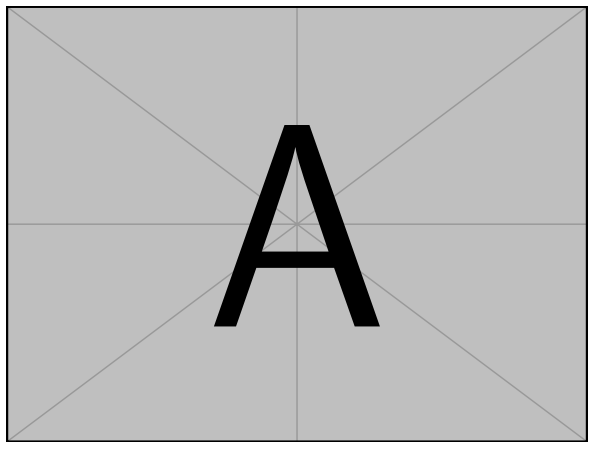
\includegraphics[width=\linewidth]{A (1).PNG}
%         \caption{partial caption figure 1}
%         \label{sub:fig1}
%     \end{subfigure}
%     \hfill
%     \begin{subfigure}[b]{0.4\textwidth}
%         \centering
%         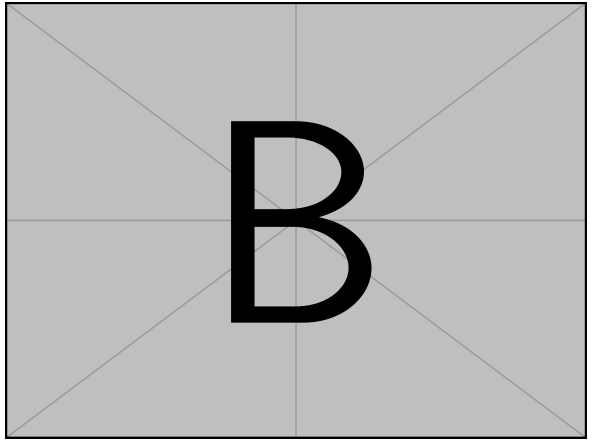
\includegraphics[width=\linewidth]{B (1).PNG}
%         \caption{partial caption figure 2}
%         \label{sub:fig2}
%     \end{subfigure}
%     \hfill
%     \begin{subfigure}[b]{0.4\textwidth}
%         \centering
%         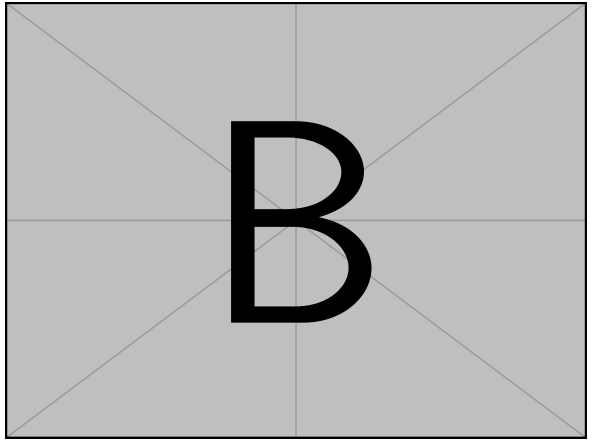
\includegraphics[width=\linewidth]{B (1).PNG}
%         \caption{Output 3}
%         \label{sub:fig3}
%     \end{subfigure}
    
%     \caption{Total caption}
%     \label{name_label}
% \end{figure}
\begin{figure}[htbp]
    \centering
    % Subfigure A
    \begin{subfigure}[b]{0.31\textwidth}
        \centering
        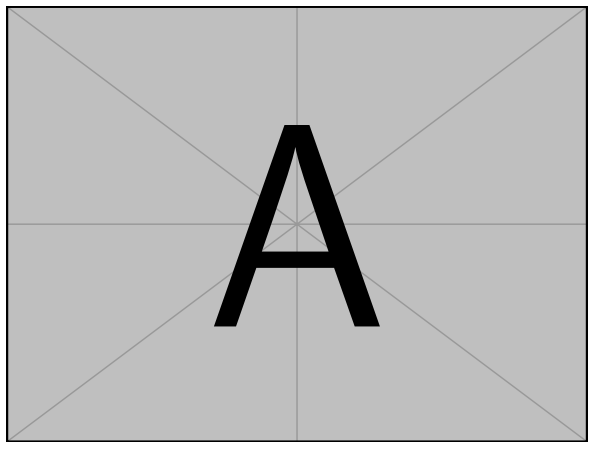
\includegraphics[width=\linewidth]{A (1).PNG}
        \caption{Output A}
        \label{sub:output_a}
    \end{subfigure}
    \hfill % Adds horizontal stretching space between the figures
    % Subfigure B
    \begin{subfigure}[b]{0.31\textwidth}
        \centering
        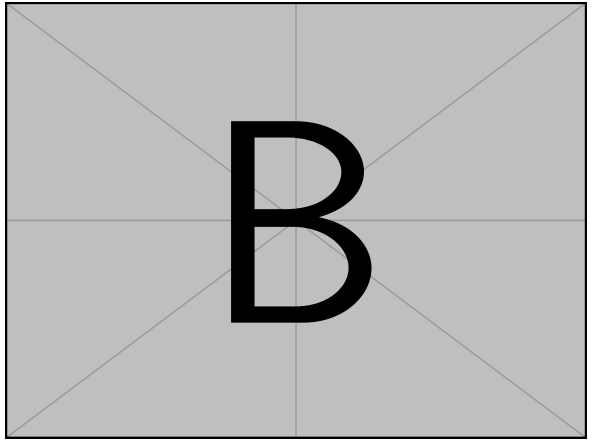
\includegraphics[width=\linewidth]{B (1).PNG}
        \caption{Output B}
        \label{sub:output_b}
    \end{subfigure}
    \hfill % Adds horizontal stretching space between the figures
    % Subfigure C
    \begin{subfigure}[b]{0.31\textwidth}
        \centering
        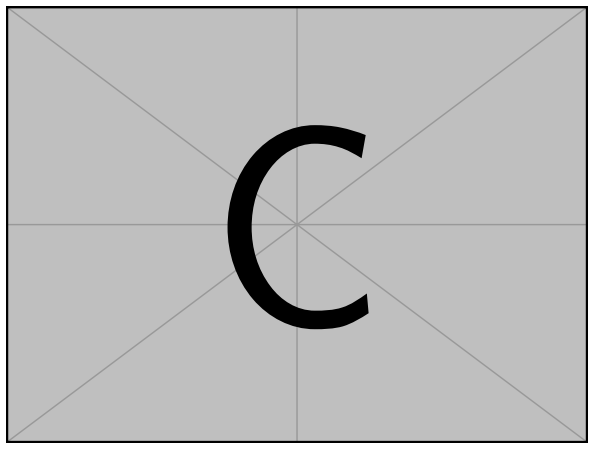
\includegraphics[width=\linewidth]{C (1).PNG}
        \caption{Output C}
        \label{sub:output_c}
    \end{subfigure}

    % Main overall caption
    \input{} % Blank layout container placeholder if needed
    \caption{Comparison of three rendering outputs.}
    \label{fig:comparison}
\end{figure}

\noindent Figure 1 compares three different rendering outputs arranged in a single row.

\section{Conclusion}

Image synthesis combines \underline{mathematical precision}, algorithmic design, and efficient implementation. As scene complexity increases, choosing the appropriate method becomes critical for balancing quality and performance.

\end{document}